\documentclass[a4paper]{article}

\usepackage[eng,exjobb]{KTHEEtitlepage}
\usepackage[cp1252]{inputenc}
\usepackage[english]{babel}
\usepackage{fancyhdr}
\usepackage{graphicx}
\usepackage[table,xcdraw]{xcolor}
\usepackage{float}
\usepackage{adjustbox}
\usepackage{ amssymb }
\usepackage{hyperref}
\usepackage{cite}

\pagestyle{fancy}
\fancyhf{}
\rhead{}
\lhead{Sound validation of the clock-shift of the Manx shearwater}
\rfoot{Page \thepage}


\begin{document}

                \ititle{Research Project}
              % \isubtitle{Julian Main, Lucas Van Berkel, Yorick De Boer, Amor Frans} % Optional
                \idate{Januari 2016}
                \irefnr{}
                \iauthor{\large{Sound validation of the clock-shift of the Manx shearwater}}
                
                \makeititle

\newpage

%%%%%%%%%%%%%%%%%%
\tableofcontents
\newpage
%%%%%%%%%%%%%%%%%%
\begin{abstract}
    Bla bla blablabla bla bla bla blablablblabla bla blalblablalblalblalbablablalbblalblablbalablbalb blba bla bla b alblblbla bla bla bla bla blab alb alb alb alb alb albbla bla bla bla bla bla bla bla lb alb albblb alb blb alb bla blb alb 
\end{abstract}
%%%%%%%%%%%%%%%%%%
\addcontentsline{toc}{section}{Introduction}
\section*{Introduction}
The research conducted here is commissioned by the Institute for Biodiversity and Ecosystem Dynamics. The institute is represented by Oliver Padget, a PhD student of the university of Oxford, helped by the dutch associate dr. ir. Emiel van Loon, Assistant Professor on statistical ecology. The project has been conducted last year by a different group, but the results were unable to give a satisfying answer to the main question of the institute.\\ \\
The subject of the project is to determine if a clock-shift has occurred on Manx shearwaters in an experiment held last summer in 2015. The experiment manipulated 8 Manx shearwaters into shifting its biological clock. The Manx Shearwater is a black and white seabird which nests in burrows. This bird nests on islands in the northeast Atlantic. In July, after the breeding period, the birds will migrate to the South-Atlantic and will return again in March the following year. During the breeding period one of the parents will stay with the eggs during a period of 7 to 12 days, while the other parent will search for food. After these 7-12 days the parents will swap roles.\\ \\ 
In order to test if the bird navigates over sea with the sun, the tested birds were manipulated, changing their endogenous clock four hours forwards or backwards. The clock-shift is a good test because if the Manx shearwater uses the sun as a compass then the bird needs a precise endogenous clock to navigate. After the clock-shifting has occurred, the birds were released some distance from their burrows on sea with GPS-tracking, to see what kind of path the birds took, returning to their burrows. To prove the clock-shifting has successfully occurred, some birds were manipulated the same way, but with a microphone in the burrow. If the Manx shearwater was clock-shifted, the researchers presumed its sound-pattern would change the same way. The main question of this research was to prove whether it was possible to show that the bird was successfully manipulated through the audio recordings.\\ \\
Audio recordings of 8 different birds were provided. Each microphone of each bird produced 9 audio files. One audio file for every day of the experiment. Last year the same research was conducted by another group. This group calculated the most dominant frequency, the activity over a period of time using the amplitude as threshold, the average amplitude over a period of time and the band power. Five minutes was the chosen step time, so every interval provided enough information to calculate each feature. The result of the previous research concluded that the results were not reliable enough to determine whether the birds were clock-shifted or not.\\ \\


%%%%%%%%%%%%%%%%%%
\addcontentsline{toc}{section}{Problem}
\section*{Problem description}
As stated before, the main subject was to determine if the clock-shift had worked. Recordings were made in 8 burrows. In each burrow the clockshift was executed. Two types of clock-shifts were used: a 4 hour forward shift(shift-fast), and a 4 hour shift backward shift(shift-slow). The recording in each burrow was approximately 24 hours for 9 days. For the first six days the time when the light was on, would match the time when the sun was up. In the last three days the clock would be shifted backwards or forward. The recordings were not complete for all burrows.
\begin{table}[H]
    \centering

\begin{tabular}{l|
>{\columncolor[HTML]{FFCE93}}c 
>{\columncolor[HTML]{FFCE93}}c 
>{\columncolor[HTML]{FFCE93}}c 
>{\columncolor[HTML]{FFCE93}}c 
>{\columncolor[HTML]{FFCE93}}c 
>{\columncolor[HTML]{FFCE93}}c 
>{\columncolor[HTML]{FFCCC9}}c 
>{\columncolor[HTML]{FFCCC9}}c 
>{\columncolor[HTML]{FFCCC9}}c }
burrow & \cellcolor[HTML]{FFFFFF}{\color[HTML]{F56B00} 16/6} & \cellcolor[HTML]{FFFFFF}{\color[HTML]{F56B00} 17/6} & \cellcolor[HTML]{FFFFFF}{\color[HTML]{F56B00} 18/6} & \cellcolor[HTML]{FFFFFF}{\color[HTML]{F56B00} 19/6} & \cellcolor[HTML]{FFFFFF}{\color[HTML]{F56B00} 20/6} & \cellcolor[HTML]{FFFFFF}{\color[HTML]{F56B00} 21//6} & \cellcolor[HTML]{FFFFFF}{\color[HTML]{CB0000} 22/6} & \cellcolor[HTML]{FFFFFF}{\color[HTML]{CB0000} 23/6} & \cellcolor[HTML]{FFFFFF}{\color[HTML]{CB0000} 24/6} \\ \hline
F:B73  & $\checkmark$                                        & $\checkmark$                                        & $\checkmark$*                                       & $\checkmark$                                        & $\checkmark$                                        & $\checkmark$*                                        & {\color[HTML]{CB0000} $\checkmark$}                 & {\color[HTML]{CB0000} $\checkmark$}                 & {\color[HTML]{CB0000} $\checkmark$}                 \\
S:B151 & $\times$                                            & $\times$                                            & $\times$                                            & $\times$                                            & $\times$                                            & $\times$                                             & {\color[HTML]{CB0000} $\times$}                     & {\color[HTML]{CB0000} $\times$}                     & {\color[HTML]{CB0000} $\checkmark$}                 \\
F:B174 & $\checkmark$                                        & $\checkmark$                                        & $\checkmark$*                                       & $\checkmark$                                        & $\checkmark$                                        & \textendash                                          & {\color[HTML]{CB0000} \textendash}                  & {\color[HTML]{CB0000} $\checkmark$}                 & {\color[HTML]{CB0000} $\checkmark$}                 \\
S:B179 & $\checkmark$                                        & $\checkmark$                                        & \textendash                                         & $\checkmark^+$                                      & $\checkmark$                                        & $\checkmark$                                         & {\color[HTML]{CB0000} $\checkmark$}                 & {\color[HTML]{CB0000} $\checkmark$}                 & {\color[HTML]{CB0000} $\checkmark$}                 \\
F:DB4  & $\checkmark$                                        & $\checkmark$                                        & $\checkmark$                                        & $\checkmark$                                        & $\checkmark$                                        & Mic                                                  & {\color[HTML]{CB0000} $\checkmark$}                 & {\color[HTML]{CB0000} $\checkmark$}                 & {\color[HTML]{CB0000} $\checkmark$}                 \\
S:DB12 & $\times$                                            & $\times$                                            & $\times$                                            & $\times$                                            & $\times$                                            & $\times$                                             & {\color[HTML]{CB0000} $\times$}                     & {\color[HTML]{CB0000} $\checkmark$}                 & {\color[HTML]{CB0000} $\checkmark$}                 \\
F:DB20 & $\checkmark$                                        & \textendash                                         & $\checkmark$                                        & $\checkmark$                                        & $\checkmark$                                        & $\checkmark$\textendash                              & {\color[HTML]{CB0000} $\checkmark$}                 & {\color[HTML]{CB0000} $\checkmark$}                 & {\color[HTML]{CB0000} $\checkmark$}                 \\
S:DB30 & $\checkmark$                                        & $\checkmark$                                        & $\checkmark$                                        & $\checkmark$                                        & \textendash                                         & $\checkmark$                                         & {\color[HTML]{CB0000} $\checkmark$}                 & {\color[HTML]{CB0000} $\checkmark$}                 & {\color[HTML]{CB0000} $\times$}                    
\end{tabular}
\caption{Table of the data given by Oliver Padget,
where $\checkmark$ means full 24 hours, $\checkmark$ \textendash means between 18 and 24 hours, $\checkmark$ * means less then 18 hours. $\times$ means no recording. Mic means that microphone was not located propperly. F means forward shift, S means backward shift.}
\end{table}
The presumption was that the clock-shift would not work immediately, comparable with a jet-lag for human beings.
It was also expected that the clock-shift would work, but in steps of 1 hour per day. This is a note that is important for the evaluation.\\\\
The main goal of this research was to validate whether the clock-shift worked based on the audio-recordings. To validate this the following sub-questions were attempted to answer:\\
 (I)    What is the activity pattern of the Manx shearwater during 24 hours in the audio recordings? \\
 (II)   What is the difference between the unshifted days and the shifted days in the activity pattern?
 
%%%%%%%%%%%%%%%%%%
\addcontentsline{toc}{section}{Strategy}
\section*{Strategy}
To determine the activity-pattern every activity in each recording was labeled. Each burrow had 24-hour of recordings for 9 days, in total approximately 216 hours of audio recording for all days. Nine burrows, so a total of 1944 hours of recordings. To solve the problem as stated before we choose to decide to follow the following strategy:\\\\
1) Preparing data \\
2) Train model to classify sounds\\
3) Abstract results from classification to usable data\\
4) Analyze results\\\\
The following chapter is a step-by-step description of how we handled the steps. 
%%%%%%%%%%%%%%%%%%
\addcontentsline{toc}{section}{Method}
\section*{Method}

\addcontentsline{toc}{subsection}{Preparing data}
\subsection*{Preparing data }

Since the audio files provided were MP3 encoded, we had to decode them to WAV format. In order to maintain the time line of every bird and audio file, each recording was split into pieces of exactly one hour long. The files had to be renamed to organize organize the data. Using the name of the files combined with the interval from the start of the original file, every audio file got its own unique start time. Each audio file, approximately $9\cdot8\cdot24=1728$ in total, was run through the the audio analysis library, delivering an array of 3600 entries long. Since the microphones of two birds did not work properly, the results of these two birds had to be discarded. 

\addcontentsline{toc}{subsection}{Train model}
\subsection*{Train model }

Since the question of the research was to determine if the pattern of the birds was shifted, We started to collect training data of distinctive sounds such as shuffling, calling and environment noise. Then let the program learn to recognize these sounds and make a vector over 24 hours of this classification. The group of last year collected trainings data of all birds combined. The results of this strategy was not so good because every burrow can differ in size and therefore the recordings can be different. Also the place of the microphone can differ in each burrow. Therefore we chose to collect trainings data for each bird separated.\\\\
To train the model to classify the sounds, an open source library for the programming language Python was used (pyAudioAnalysis). This library  uses 34 different short-period features, in order to determine if the sound tested, matches the sound classified using the K-nearest neighbours algorithm. Some of the features the program uses are the Zero Crossing Rate, Entropy of Energy and Spectral Spread. A complete overview of every feature is provided along with the code. While listening to some audio files, multiple sounds could clearly be classified. The most interesting sound was when the bird moved, the sound you get when something moves over the microphone, this sound was named 'shuffle'. Other sounds were some random microphones beeps and a constant background noise which was classified as silence. The step size this program uses was one second long, and returns the classification of every second in the tested audio file.
\\\\A preliminary test of detecting 'shuffles' in a time frame of 241 seconds concluded that 90 percent of the 'shuffles' was detected in that time frame. \\
\begin{figure}[!ht]
  \centering
    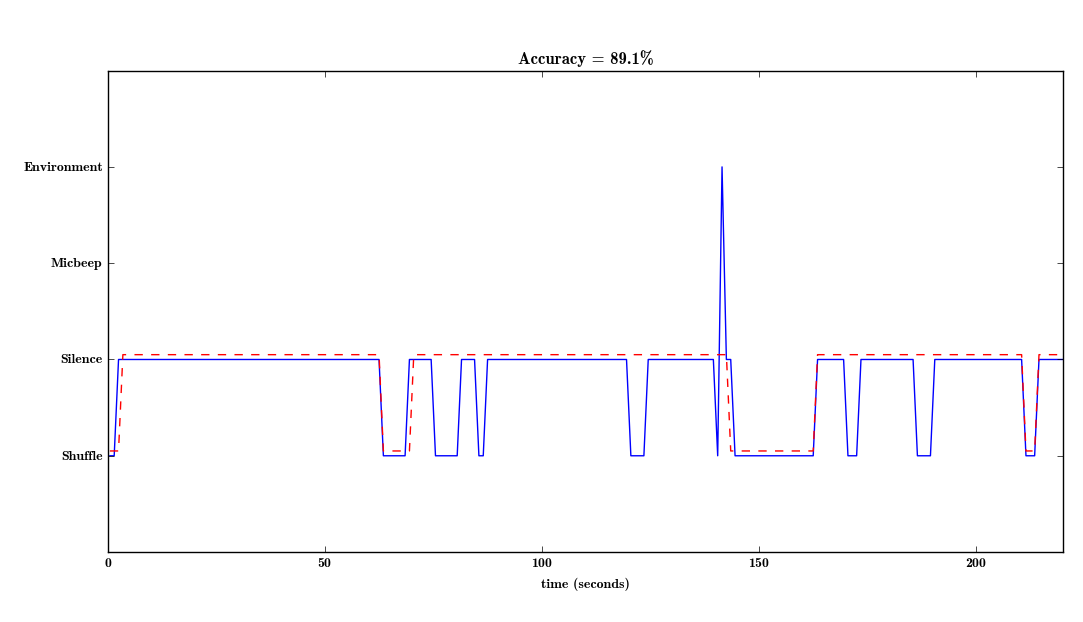
\includegraphics[width=0.9\textwidth]{accuracy_test_crop}
      \caption{Accuracy test}
\end{figure}
\\
After this we collected sound fragments for every bird separately. Every bird had a different environment so the we could not use the same training data for every bird.

\addcontentsline{toc}{subsection}{Abstract to usable data}
\subsection*{Abstract to usable data}
Every second of sound then was labeled with its class and put into an array. Next every class was labeled with a timestamp and put into CSV-files (Comma-separated values files) for every bird. The CSV-files were later put into a sqllite-database (Structured Query Language Database), in order to make it easier to retrieve data from certain time points during the analysis.

\addcontentsline{toc}{subsection}{Analyze results}
\subsection*{Analyze results}
After the data was usable there were two methods that we used to analyze the data: confidence interval test and anomaly detection.
\addcontentsline{toc}{subsubsection}{Confidence interval test}
\subsubsection*{Confidence interval test}
To validate the clockshift the shifted days must be compared with the unshifted days. We have the classifications of shuffles for each day for every hour during 24 hours. Therefore the vector of a day consist 24 variables and each variable represent the amount of shuffles in that hour. There are six vectors of the unshifted days and three vectors from the shifted day for each bird.\\\
The idea is to separate every hour and make a confidence interval for every hour using the data from the unshifted days. And then look if the same hour in the shifted day falls in that confidence interval. After this procedure the program will shift the vector of the shifted day and repeat the procedure.\\\\ 
For example if we take hour 13, we have data how many shuffles there were in hour 13 for day 16-21(unshifted days). We put all the points of hour 13 from all the six unshifted days together . So we now have a vector of length six for hour 13, representing the amount of shuffles in hour 13 for the six days. With this vector we make a confidence interval assuming the points are distributed as a t-distribution. Say the program computes the interval 800-1200. Then the program checks if  the amount of shuffles in hour 13 on the shifted day falls into that interval. So if in hour 13 on a shifted there were 900 shuffles then the programs label this hour as a 1 if the amount of shuffles in that hour is not in the interval than the programs gives that hour score 0.  The programs repeats this procedure for every hour, so at the end it computes a percentage of the hours that falls in the confidence interval.\\\\
After this whole procedure we shift the time-line of the shifted day by an hour and we do this four times. This is because the birds will not shift their activity immediately therefore we must check the shift of 0-4 hours. The expectation is that the birds will shift by ca. 1 hour per day so we want to see that the percentage of hours that falls in the confidence interval will increase by the hours of shifting. If that is the case then we can conclude that the clock-shift has worked. 

\addcontentsline{toc}{subsubsection}{Anomaly detection}
\subsubsection*{Anomaly detection}
The idea of anomaly detection is to check whether a new vector or point fit in the data that is given before. Using machine learning we can train the program to make a decision boundary to check if the new vector or point fits. So first the program needs to be trained using the trainingsdata then using an algorithm the decision boundary will be made so the new vectors can be analyzed whether it is anomalous or not.\\\\
For an anomaly detection algorithm we chose to use the least-squares kernel based method.  If there are two vectors x and y then a kernel is the space of all vectors in x that will denote in the zero-vector in y. The least squares equation is an equation to compute the distance between the estimation and the real value, the idea of is that we want to minimize this distance using the algorithms and kernels. For an extensive explanation of this algorithm read this reference.*****.\\\\
For this research the trainingsdata will be the data of the amount of shuffles for each hour in all unshifted days, this are six vectors which each represent an unshifted day. Then a shifted day will be the compared vector. To validate whether the clock-shift has happened we first compare a shifted day before the shift and then after the shift. We hope to see that this vector will be flagged as anomalous before the shift because it must not fit in the unshifted day pattern and it will be flagged as not anomalous after the shift. If this is the case then we can conclude that the clock-shift worked.\\\
%%%%%%%%%%%%%%%%%%
\addcontentsline{toc}{section}{Results}
\section*{Results}

\addcontentsline{toc}{subsection}{Classification}
\subsection*{Classification}
To make the results conceivable we made a couple of different plots. With a perfect clock shifted result the pattern of activity for 24 hours would be exactly the same for all days. When there would be a shift, the difference between the shifted days and the non shifted days would then be that the pattern also shifted. \\
Unfortunately this is not the case. Although there is definitely a pattern among the activity patterns of some birds, other birds do not show a clear daily pattern. Two of the total six tested birds show a pattern which is visible when plotted.

\begin{figure}[H]
  \centering
    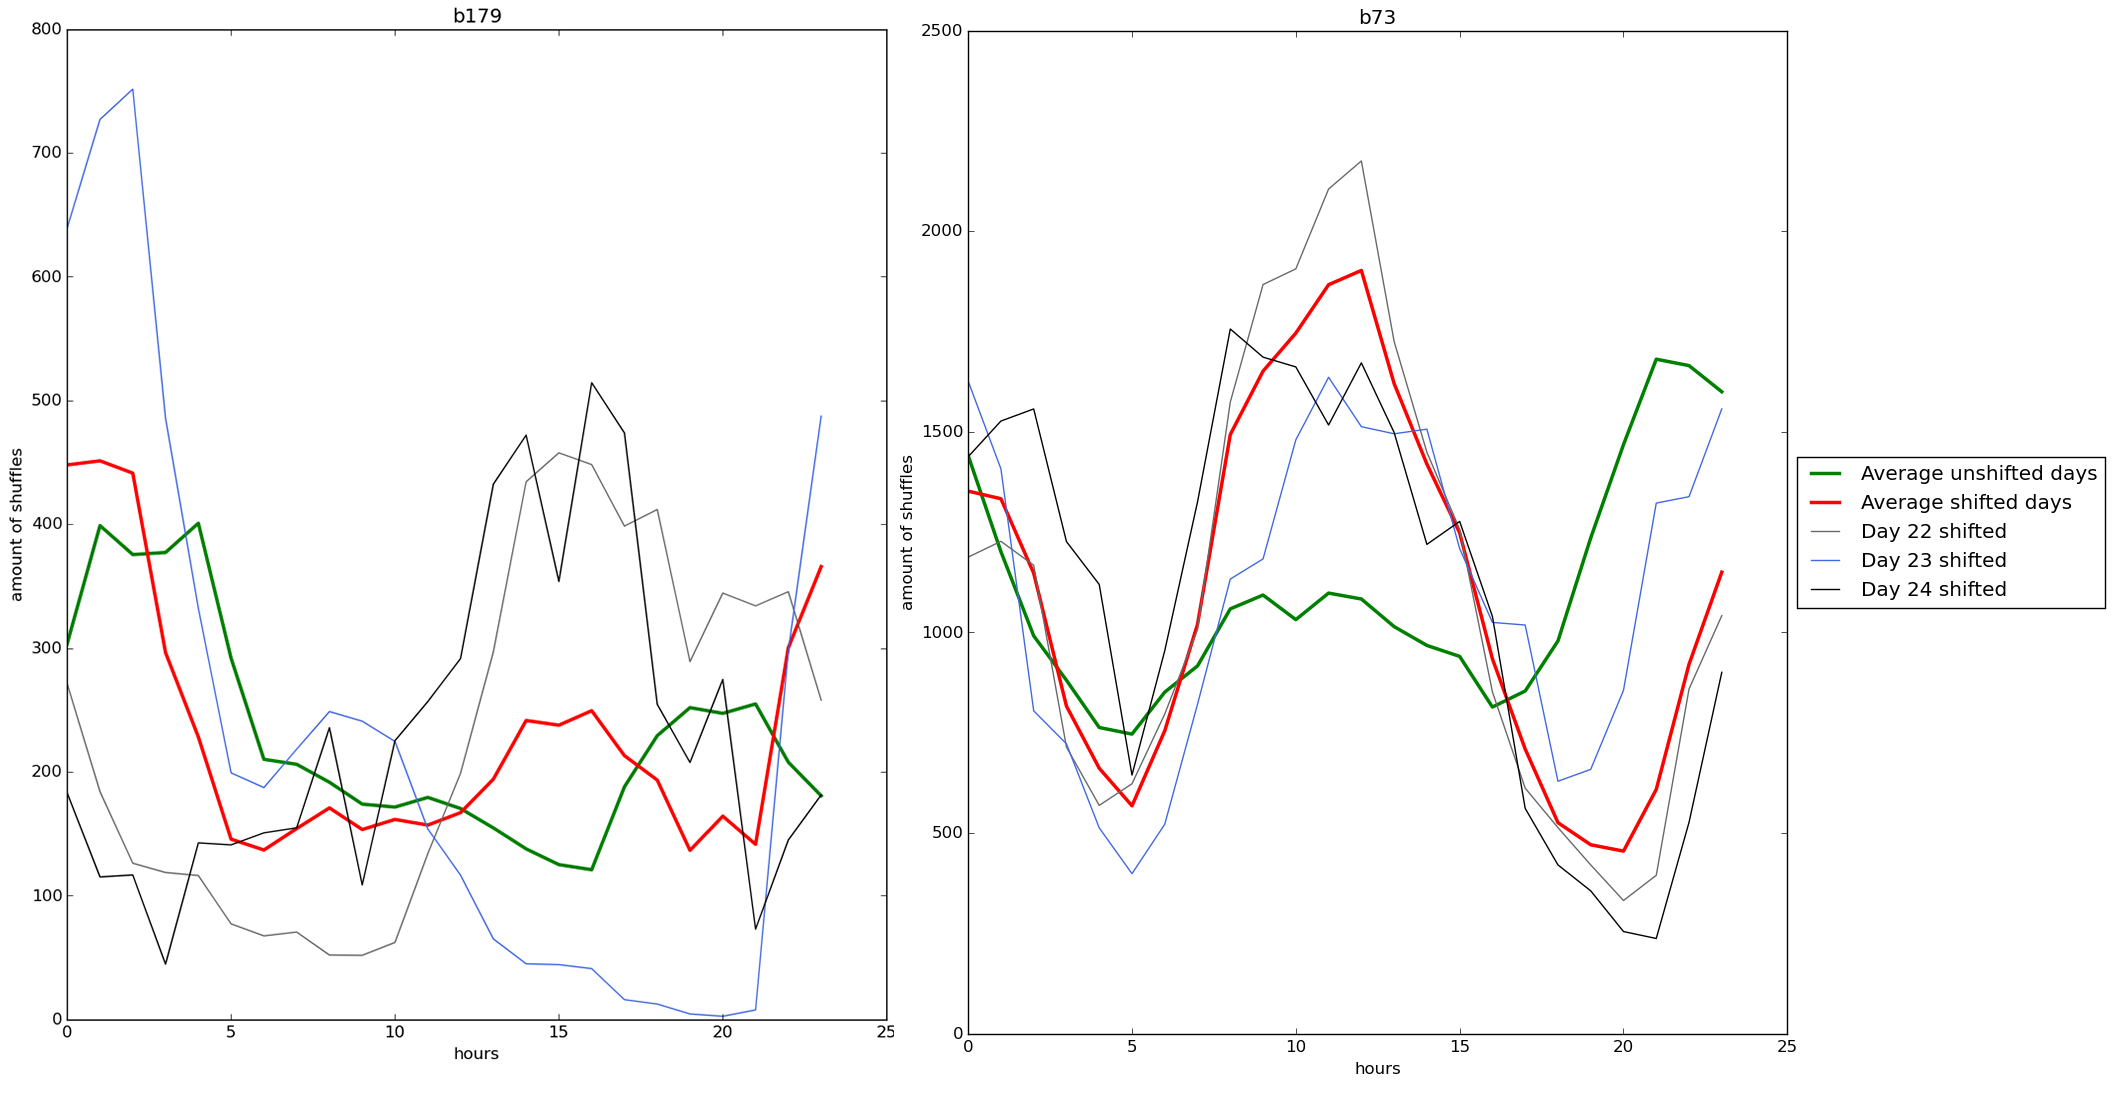
\includegraphics[width=1\textwidth]{b179_b73_merged}
      \caption{Comparison of shifted vs nonshifted days of bird b179 and b73}
\end{figure}

To find out how the average of the non shifted days represents the the real value, a min-max plot was made.
\begin{figure}[H]
  \centering
    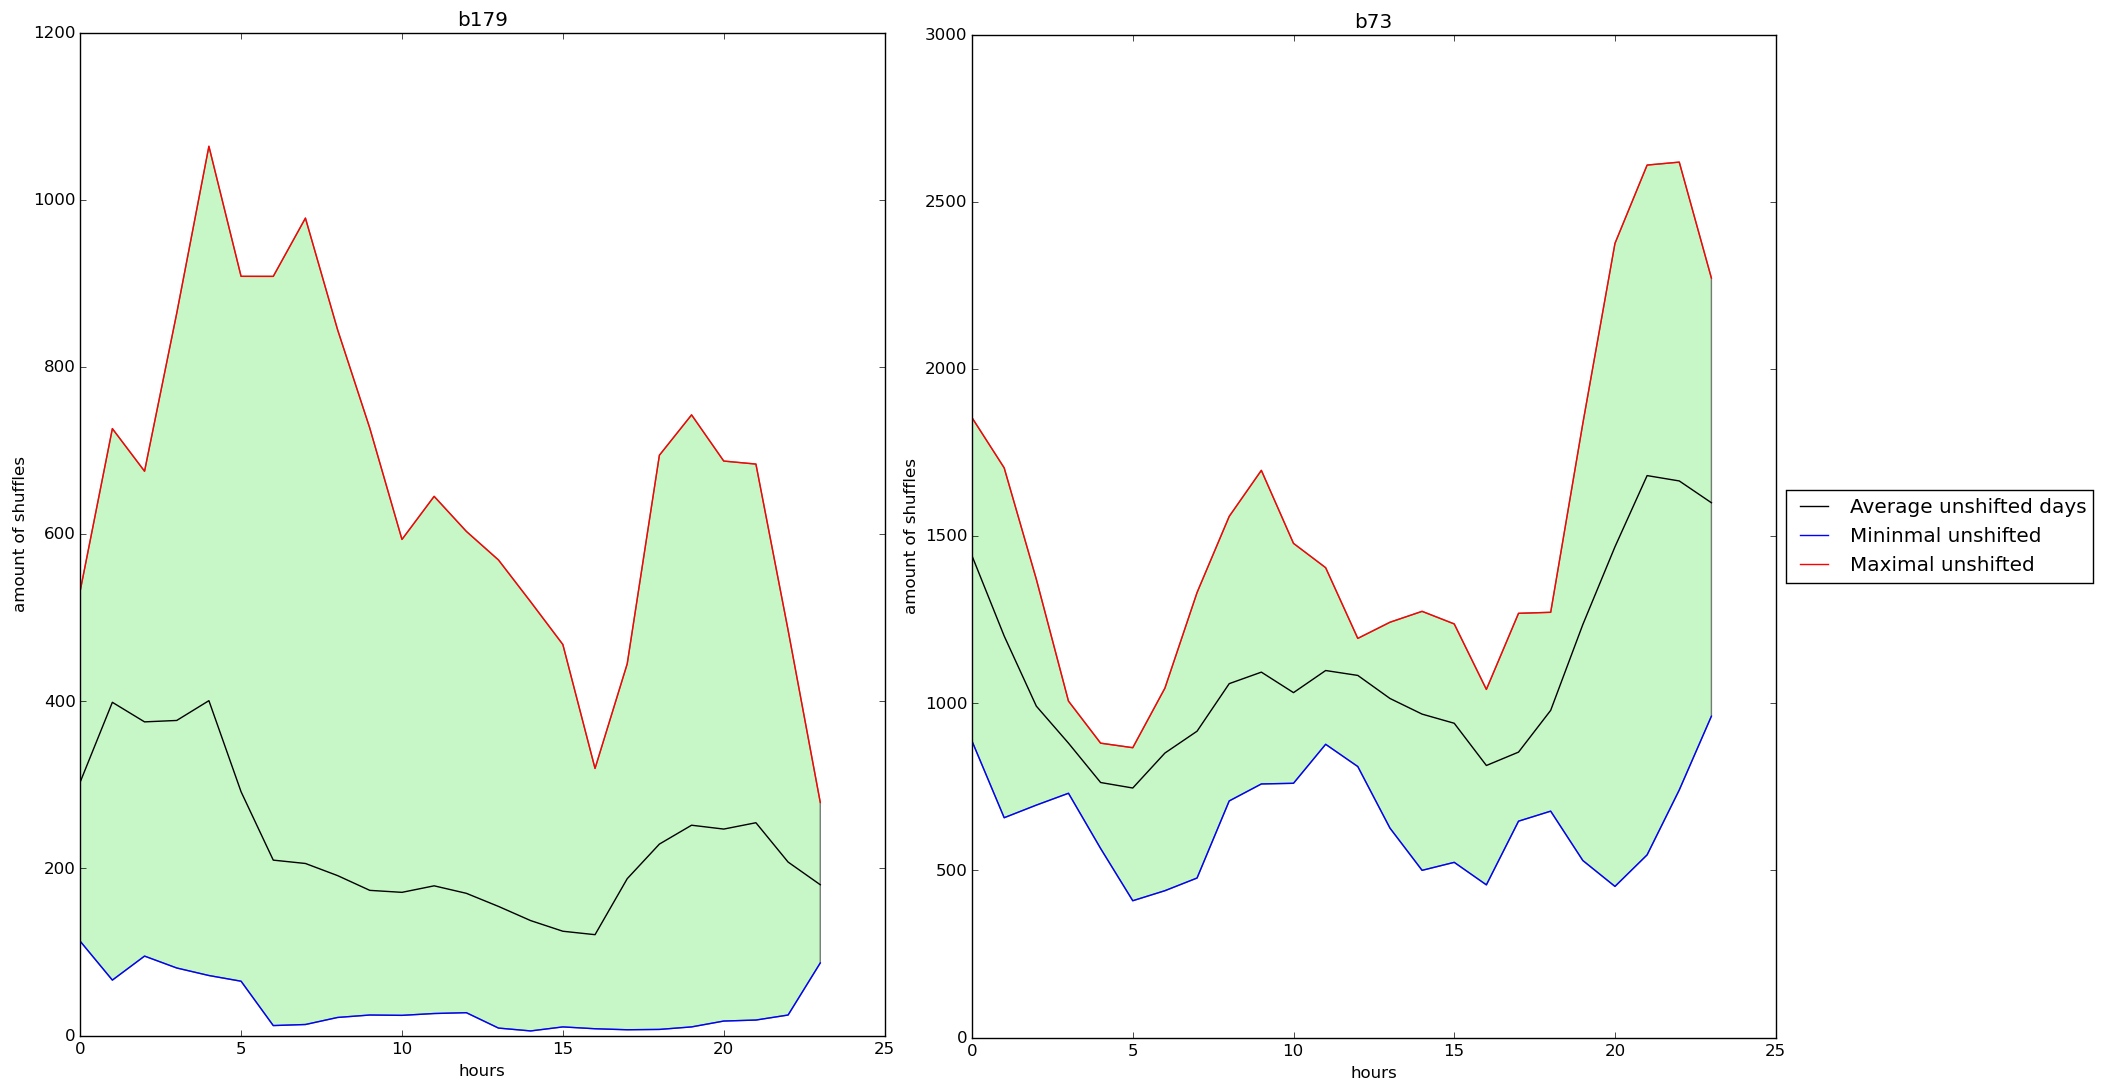
\includegraphics[width=1\textwidth]{b179_b73_merged_surface}
      \caption{Minimal and maximal values of non shifted days bird b179 and b73}
\end{figure}
It can be seen that there is a significant difference between these two birds. While the min and max values from the b73 bird are quite close the the average, the values of the b179 bird are much further apart.
\addcontentsline{toc}{subsection}{Confidence interval Test}
\subsection*{Confidence interval Test}
As stated before, we ran a test to validate whether the pattern from the shifted days and unshifted days differ significantly. This are the results of the confidence interval test:\\
\begin{table}[H]
\centering
\resizebox{\textwidth}{!}{%
\begin{tabular}{lllllllllll}
\hline
\multicolumn{1}{|l|}{} & \multicolumn{5}{l|}{\textbf{Day 22}} & \multicolumn{5}{l|}{\textbf{Day 23}} \\ \hline
\multicolumn{1}{|l|}{\textit{hours of shifting}} & \multicolumn{1}{l|}{\textit{0}} & \multicolumn{1}{l|}{\textit{1}} & \multicolumn{1}{l|}{\textit{2}} & \multicolumn{1}{l|}{\textit{3}} & \multicolumn{1}{l|}{\textit{4}} & \multicolumn{1}{l|}{\textit{0}} & \multicolumn{1}{l|}{\textit{1}} & \multicolumn{1}{l|}{\textit{2}} & \multicolumn{1}{l|}{\textit{3}} & \multicolumn{1}{l|}{\textit{4}} \\ \hline
\multicolumn{1}{|l|}{\textbf{b73}} & \multicolumn{1}{l|}{\cellcolor[HTML]{BBDAFF}54.167\%} & \multicolumn{1}{l|}{\cellcolor[HTML]{EA6D67}45.83\%} & \multicolumn{1}{l|}{\cellcolor[HTML]{EA6D67}37.5\%} & \multicolumn{1}{l|}{\cellcolor[HTML]{EA6D67}29.17\%} & \multicolumn{1}{l|}{\cellcolor[HTML]{EA6D67}33.33\%} & \multicolumn{1}{l|}{\cellcolor[HTML]{BBDAFF}29.17\%} & \multicolumn{1}{l|}{\cellcolor[HTML]{EA6D67}25.0\%} & \multicolumn{1}{l|}{\cellcolor[HTML]{4ECF94}41.67\%} & \multicolumn{1}{l|}{\cellcolor[HTML]{4ECF94}45.83\%} & \multicolumn{1}{l|}{\cellcolor[HTML]{4ECF94}37.5\%} \\ \hline
\multicolumn{1}{|l|}{\textbf{b174}} & \multicolumn{1}{l|}{\cellcolor[HTML]{BBDAFF}0.0\%} & \multicolumn{1}{l|}{\cellcolor[HTML]{4ECF94}8.33\%} & \multicolumn{1}{l|}{\cellcolor[HTML]{4ECF94}12.55\%} & \multicolumn{1}{l|}{\cellcolor[HTML]{4ECF94}8.33\%} & \multicolumn{1}{l|}{\cellcolor[HTML]{4ECF94}4.167\%} & \multicolumn{1}{l|}{\cellcolor[HTML]{BBDAFF}50.0\%} & \multicolumn{1}{l|}{\cellcolor[HTML]{4ECF94}58.33\%} & \multicolumn{1}{l|}{\cellcolor[HTML]{FFFE65}50.0\%} & \multicolumn{1}{l|}{\cellcolor[HTML]{EA6D67}45.83\%} & \multicolumn{1}{l|}{\cellcolor[HTML]{FFFE65}50.0\%} \\ \hline
\multicolumn{1}{|l|}{\textbf{b179}} & \multicolumn{1}{l|}{\cellcolor[HTML]{BBDAFF}75.0\%} & \multicolumn{1}{l|}{\cellcolor[HTML]{4ECF94}79.17\%} & \multicolumn{1}{l|}{\cellcolor[HTML]{FFFE65}75.0\%} & \multicolumn{1}{l|}{\cellcolor[HTML]{4ECF94}87.50\%} & \multicolumn{1}{l|}{\cellcolor[HTML]{FFFE65}75.0\%} & \multicolumn{1}{l|}{\cellcolor[HTML]{BBDAFF}79.17\%} & \multicolumn{1}{l|}{\cellcolor[HTML]{4ECF94}83.33\%} & \multicolumn{1}{l|}{\cellcolor[HTML]{EA6D67}75.0\%} & \multicolumn{1}{l|}{\cellcolor[HTML]{FFFE65}79.17\%} & \multicolumn{1}{l|}{\cellcolor[HTML]{FFFE65}79.17\%} \\ \hline
\multicolumn{1}{|l|}{\textbf{DB4}} & \multicolumn{1}{l|}{\cellcolor[HTML]{BBDAFF}50.0\%} & \multicolumn{1}{l|}{\cellcolor[HTML]{FFFE65}50.0\%} & \multicolumn{1}{l|}{\cellcolor[HTML]{FFFE65}50.0\%} & \multicolumn{1}{l|}{\cellcolor[HTML]{4ECF94}54.17\%} & \multicolumn{1}{l|}{\cellcolor[HTML]{4ECF94}54.17\%} & \multicolumn{1}{l|}{\cellcolor[HTML]{BBDAFF}37.50\%} & \multicolumn{1}{l|}{\cellcolor[HTML]{4ECF94}54.17\%} & \multicolumn{1}{l|}{\cellcolor[HTML]{4ECF94}41.67\%} & \multicolumn{1}{l|}{\cellcolor[HTML]{4ECF94}50.0\%} & \multicolumn{1}{l|}{\cellcolor[HTML]{4ECF94}41.67\%} \\ \hline
\multicolumn{1}{|l|}{\textbf{DB20}} & \multicolumn{1}{l|}{\cellcolor[HTML]{BBDAFF}100.0\%} & \multicolumn{1}{l|}{\cellcolor[HTML]{EA6D67}95.83\%} & \multicolumn{1}{l|}{\cellcolor[HTML]{EA6D67}91.67\%} & \multicolumn{1}{l|}{\cellcolor[HTML]{EA6D67}87.5\%} & \multicolumn{1}{l|}{\cellcolor[HTML]{EA6D67}95.83\%} & \multicolumn{1}{l|}{\cellcolor[HTML]{BBDAFF}95.83\%} & \multicolumn{1}{l|}{\cellcolor[HTML]{4ECF94}100\%} & \multicolumn{1}{l|}{\cellcolor[HTML]{FFFE65}95.83\%} & \multicolumn{1}{l|}{\cellcolor[HTML]{EA6D67}91.67\%} & \multicolumn{1}{l|}{\cellcolor[HTML]{EA6D67}91.67\%} \\ \hline
\multicolumn{1}{|l|}{\textbf{DB30}} & \multicolumn{1}{l|}{\cellcolor[HTML]{BBDAFF}50.0\%} & \multicolumn{1}{l|}{\cellcolor[HTML]{EA6D67}45.83\%} & \multicolumn{1}{l|}{\cellcolor[HTML]{EA6D67}45.83\%} & \multicolumn{1}{l|}{\cellcolor[HTML]{EA6D67}37.5\%} & \multicolumn{1}{l|}{\cellcolor[HTML]{EA6D67}41.67\%} & \multicolumn{1}{l|}{\cellcolor[HTML]{BBDAFF}25.0\%} & \multicolumn{1}{l|}{\cellcolor[HTML]{FFFE65}25.0\%} & \multicolumn{1}{l|}{\cellcolor[HTML]{FFFE65}25.0\%} & \multicolumn{1}{l|}{\cellcolor[HTML]{EA6D67}16.67\%} & \multicolumn{1}{l|}{\cellcolor[HTML]{EA6D67}8.33\%} \\ \hline
\multicolumn{1}{|l|}{} & \multicolumn{5}{l|}{\textbf{Day 24}} & \multicolumn{5}{l}{\cellcolor[HTML]{FFFFFF}} \\ \cline{1-6}
\multicolumn{1}{|l|}{\textit{hours of shifting}} & \multicolumn{1}{l|}{\textit{0}} & \multicolumn{1}{l|}{\textit{1}} & \multicolumn{1}{l|}{\textit{2}} & \multicolumn{1}{l|}{\textit{3}} & \multicolumn{1}{l|}{\textit{4}} & \multicolumn{5}{l}{\cellcolor[HTML]{FFFFFF}} \\ \cline{1-6}
\multicolumn{1}{|l|}{\textbf{b73}} & \multicolumn{1}{l|}{\cellcolor[HTML]{BBDAFF}25.0\%} & \multicolumn{1}{l|}{\cellcolor[HTML]{4ECF94}29.17\%} & \multicolumn{1}{l|}{\cellcolor[HTML]{4ECF94}29.17\%} & \multicolumn{1}{l|}{\cellcolor[HTML]{4ECF94}45.83\%} & \multicolumn{1}{l|}{\cellcolor[HTML]{4ECF94}37.5\%} & \multicolumn{5}{l}{\cellcolor[HTML]{FFFFFF}} \\ \cline{1-6}
\multicolumn{1}{|l|}{\textbf{b174}} & \multicolumn{1}{l|}{\cellcolor[HTML]{BBDAFF}62.5\%} & \multicolumn{1}{l|}{\cellcolor[HTML]{EA6D67}62.5\%} & \multicolumn{1}{l|}{\cellcolor[HTML]{EA6D67}58.33\%} & \multicolumn{1}{l|}{\cellcolor[HTML]{EA6D67}50.0\%} & \multicolumn{1}{l|}{\cellcolor[HTML]{EA6D67}54.17\%} & \multicolumn{5}{l}{\cellcolor[HTML]{FFFFFF}} \\ \cline{1-6}
\multicolumn{1}{|l|}{\textbf{b179}} & \multicolumn{1}{l|}{\cellcolor[HTML]{BBDAFF}83.33\%} & \multicolumn{1}{l|}{\cellcolor[HTML]{FFFE65}83.33\%} & \multicolumn{1}{l|}{\cellcolor[HTML]{4ECF94}87.5\%} & \multicolumn{1}{l|}{\cellcolor[HTML]{FFFE65}83,33\%} & \multicolumn{1}{l|}{\cellcolor[HTML]{4ECF94}87.5\%} & \multicolumn{5}{l}{\cellcolor[HTML]{FFFFFF}} \\ \cline{1-6}
\multicolumn{1}{|l|}{\textbf{DB4}} & \multicolumn{1}{l|}{\cellcolor[HTML]{BBDAFF}58.33\%} & \multicolumn{1}{l|}{\cellcolor[HTML]{FFFE65}58.33\%} & \multicolumn{1}{l|}{\cellcolor[HTML]{EA6D67}54.17\%} & \multicolumn{1}{l|}{\cellcolor[HTML]{EA6D67}50.0\%} & \multicolumn{1}{l|}{\cellcolor[HTML]{EA6D67}50.0\%} & \multicolumn{5}{l}{\cellcolor[HTML]{FFFFFF}} \\ \cline{1-6}
\multicolumn{1}{|l|}{\textbf{DB20}} & \multicolumn{1}{l|}{\cellcolor[HTML]{BBDAFF}87.50\%} & \multicolumn{1}{l|}{\cellcolor[HTML]{EA6D67}83.33\%} & \multicolumn{1}{l|}{\cellcolor[HTML]{4ECF94}91.67\%} & \multicolumn{1}{l|}{\cellcolor[HTML]{4ECF94}91.67\%} & \multicolumn{1}{l|}{\cellcolor[HTML]{EA6D67}83.33\%} & \multicolumn{5}{l}{\cellcolor[HTML]{FFFFFF}} \\ \cline{1-6}
\multicolumn{1}{|l|}{\textbf{DB30}} & \multicolumn{1}{l|}{\cellcolor[HTML]{BBDAFF}8.33\%} & \multicolumn{1}{l|}{\cellcolor[HTML]{FFFE65}8.33\%} & \multicolumn{1}{l|}{\cellcolor[HTML]{FFFE65}8.33\%} & \multicolumn{1}{l|}{\cellcolor[HTML]{FFFE65}8.33\%} & \multicolumn{1}{l|}{\cellcolor[HTML]{FFFE65}8.33\%} & \multicolumn{5}{l}{\multirow{-8}{*}{\cellcolor[HTML]{FFFFFF}}} \\ \cline{1-6}
\multicolumn{11}{l}{}
\end{tabular}
}
\caption{Results of the confidence interval test. \small{\emph{Green: percentage of the of the hours that falls in the confidence interval increases, 
red: percentage of the of the hours that falls in the confidence interval decreases, Yellow: percentage of the of the hours that falls in the confidence interval stays the same }}}
\label{my-label}
\end{table}
Here the each row represent a bird and the days 21,22 and 23 are the shifted days. The hours of shifting is the hours we shift the timeline of the shifted day. In the green cells the percentage of hours that falls in the confidence interval increases comparing to the base case where no shift has been made yet, in the red cells the percentage decreases and in the yellow cells the percentage stays the same. If the clock-shift worked then the percentage must increases.\\\\
Because the birds will not change their behaviour immediately after the clock shift the columns shifted-hours 1,2 and 3 are more important for day 22. In the table 3 of the 6 birds percentage increased for day 22 for the columns shifted-hours 1,2 or 3, which are bird b174, b179 and DB4. For day 23 the shifted hours 2,3,4 are more important assuming the birds is adapting  to the clock-shift better now. Here we can see that 2 of the 6 birds percentage increased at in one of the three important hours. For the last day the important columns are the shifted-hours 3 and 4, assuming again that the bird has now adapt more to the clock-shift. Here we also see 2 of the 6 birds percentage increasing.\\\\
Remark that day 24 is the most import day to compare because at this day we will assume that the bird has fully adapt tot the clock-shift. Interesting to see is that in day 24 of bird b73 all percentage increases, this is a sign that the clock-shift has worked on bird b73. A similar pattern we can see for bird b179 for day 24. Bird DB20 looks like he is not fully adapted yet but still shifted 3 hours.\\\\
3 of the 6 birds shows are showing good results, so there are signs that the clock-shift has worked but it is not significant enough to conclude that with confidence. 


\addcontentsline{toc}{subsection}{Anomaly detection}
\subsection*{Anomaly detection}
As stated in the method, anomaly detection will flag vectors as being anomalous if they do not fit a certain a group of data(cluster), which means that the pattern of activity differs. The vector of the activity of a shifted day will be compared with the cluster of the unshifted days using the least squared kernel-based method. If the compared vector exceeds a certain threshold than the vector will be flagged as anomalous. Due to the birds will not shift immediately we defined the clock-shift by steps of 1 hour. The results are as following:\\
\begin{table}[H]
\centering
\label{my-label}
\begin{tabular}{llllllllllllllll}
\hline
\multicolumn{1}{|l|}{} & \multicolumn{5}{l|}{\textbf{Day 22}} & \multicolumn{5}{l|}{\textbf{Day 23}} & \multicolumn{5}{l|}{\textbf{Day 24}} \\ \hline
\multicolumn{1}{|l|}{\textit{hours of shifting}} & \multicolumn{1}{l|}{\textit{0}} & \multicolumn{1}{l|}{\textit{1}} & \multicolumn{1}{l|}{\textit{2}} & \multicolumn{1}{l|}{\textit{3}} & \multicolumn{1}{l|}{\textit{4}} & \multicolumn{1}{l|}{\textit{0}} & \multicolumn{1}{l|}{\textit{1}} & \multicolumn{1}{l|}{\textit{2}} & \multicolumn{1}{l|}{\textit{3}} & \multicolumn{1}{l|}{\textit{4}} & \multicolumn{1}{l|}{\textit{0}} & \multicolumn{1}{l|}{\textit{1}} & \multicolumn{1}{l|}{\textit{2}} & \multicolumn{1}{l|}{\textit{3}} & \multicolumn{1}{l|}{\textit{4}} \\ \hline
\multicolumn{1}{|l|}{\textbf{b73}} & \multicolumn{1}{l|}{\cellcolor[HTML]{4ECF94}} & \multicolumn{1}{l|}{\cellcolor[HTML]{4ECF94}} & \multicolumn{1}{l|}{\cellcolor[HTML]{EA6D67}} & \multicolumn{1}{l|}{\cellcolor[HTML]{EA6D67}} & \multicolumn{1}{l|}{\cellcolor[HTML]{4ECF94}} & \multicolumn{1}{l|}{\cellcolor[HTML]{4ECF94}} & \multicolumn{1}{l|}{\cellcolor[HTML]{4ECF94}} & \multicolumn{1}{l|}{\cellcolor[HTML]{4ECF94}} & \multicolumn{1}{l|}{\cellcolor[HTML]{4ECF94}} & \multicolumn{1}{l|}{\cellcolor[HTML]{4ECF94}} & \multicolumn{1}{l|}{\cellcolor[HTML]{EA6D67}} & \multicolumn{1}{l|}{\cellcolor[HTML]{EA6D67}} & \multicolumn{1}{l|}{\cellcolor[HTML]{EA6D67}} & \multicolumn{1}{l|}{\cellcolor[HTML]{EA6D67}} & \multicolumn{1}{l|}{\cellcolor[HTML]{EA6D67}} \\ \hline
\multicolumn{1}{|l|}{\textbf{b174}} & \multicolumn{1}{l|}{\cellcolor[HTML]{EA6D67}} & \multicolumn{1}{l|}{\cellcolor[HTML]{EA6D67}} & \multicolumn{1}{l|}{\cellcolor[HTML]{EA6D67}} & \multicolumn{1}{l|}{\cellcolor[HTML]{EA6D67}} & \multicolumn{1}{l|}{\cellcolor[HTML]{EA6D67}} & \multicolumn{1}{l|}{\cellcolor[HTML]{4ECF94}} & \multicolumn{1}{l|}{\cellcolor[HTML]{4ECF94}} & \multicolumn{1}{l|}{\cellcolor[HTML]{4ECF94}} & \multicolumn{1}{l|}{\cellcolor[HTML]{4ECF94}} & \multicolumn{1}{l|}{\cellcolor[HTML]{4ECF94}} & \multicolumn{1}{l|}{\cellcolor[HTML]{4ECF94}} & \multicolumn{1}{l|}{\cellcolor[HTML]{4ECF94}} & \multicolumn{1}{l|}{\cellcolor[HTML]{4ECF94}} & \multicolumn{1}{l|}{\cellcolor[HTML]{4ECF94}} & \multicolumn{1}{l|}{\cellcolor[HTML]{4ECF94}} \\ \hline
\multicolumn{1}{|l|}{\textbf{b179}} & \multicolumn{1}{l|}{\cellcolor[HTML]{4ECF94}} & \multicolumn{1}{l|}{\cellcolor[HTML]{4ECF94}} & \multicolumn{1}{l|}{\cellcolor[HTML]{4ECF94}} & \multicolumn{1}{l|}{\cellcolor[HTML]{4ECF94}} & \multicolumn{1}{l|}{\cellcolor[HTML]{4ECF94}} & \multicolumn{1}{l|}{\cellcolor[HTML]{EA6D67}} & \multicolumn{1}{l|}{\cellcolor[HTML]{EA6D67}} & \multicolumn{1}{l|}{\cellcolor[HTML]{EA6D67}} & \multicolumn{1}{l|}{\cellcolor[HTML]{EA6D67}} & \multicolumn{1}{l|}{\cellcolor[HTML]{EA6D67}} & \multicolumn{1}{l|}{\cellcolor[HTML]{4ECF94}} & \multicolumn{1}{l|}{\cellcolor[HTML]{4ECF94}} & \multicolumn{1}{l|}{\cellcolor[HTML]{4ECF94}} & \multicolumn{1}{l|}{\cellcolor[HTML]{4ECF94}} & \multicolumn{1}{l|}{\cellcolor[HTML]{4ECF94}} \\ \hline
\multicolumn{1}{|l|}{\textbf{DB4}} & \multicolumn{1}{l|}{\cellcolor[HTML]{4ECF94}} & \multicolumn{1}{l|}{\cellcolor[HTML]{4ECF94}} & \multicolumn{1}{l|}{\cellcolor[HTML]{4ECF94}} & \multicolumn{1}{l|}{\cellcolor[HTML]{4ECF94}} & \multicolumn{1}{l|}{\cellcolor[HTML]{4ECF94}} & \multicolumn{1}{l|}{\cellcolor[HTML]{4ECF94}} & \multicolumn{1}{l|}{\cellcolor[HTML]{4ECF94}} & \multicolumn{1}{l|}{\cellcolor[HTML]{4ECF94}} & \multicolumn{1}{l|}{\cellcolor[HTML]{4ECF94}} & \multicolumn{1}{l|}{\cellcolor[HTML]{4ECF94}} & \multicolumn{1}{l|}{\cellcolor[HTML]{4ECF94}} & \multicolumn{1}{l|}{\cellcolor[HTML]{4ECF94}} & \multicolumn{1}{l|}{\cellcolor[HTML]{4ECF94}} & \multicolumn{1}{l|}{\cellcolor[HTML]{4ECF94}} & \multicolumn{1}{l|}{\cellcolor[HTML]{4ECF94}} \\ \hline
\multicolumn{1}{|l|}{\textbf{DB20}} & \multicolumn{1}{l|}{\cellcolor[HTML]{4ECF94}} & \multicolumn{1}{l|}{\cellcolor[HTML]{4ECF94}} & \multicolumn{1}{l|}{\cellcolor[HTML]{4ECF94}} & \multicolumn{1}{l|}{\cellcolor[HTML]{4ECF94}} & \multicolumn{1}{l|}{\cellcolor[HTML]{4ECF94}} & \multicolumn{1}{l|}{\cellcolor[HTML]{4ECF94}} & \multicolumn{1}{l|}{\cellcolor[HTML]{4ECF94}} & \multicolumn{1}{l|}{\cellcolor[HTML]{4ECF94}} & \multicolumn{1}{l|}{\cellcolor[HTML]{4ECF94}} & \multicolumn{1}{l|}{\cellcolor[HTML]{4ECF94}} & \multicolumn{1}{l|}{\cellcolor[HTML]{4ECF94}} & \multicolumn{1}{l|}{\cellcolor[HTML]{4ECF94}} & \multicolumn{1}{l|}{\cellcolor[HTML]{4ECF94}} & \multicolumn{1}{l|}{\cellcolor[HTML]{4ECF94}} & \multicolumn{1}{l|}{\cellcolor[HTML]{4ECF94}} \\ \hline
\multicolumn{1}{|l|}{\textbf{DB30}} & \multicolumn{1}{l|}{\cellcolor[HTML]{EA6D67}} & \multicolumn{1}{l|}{\cellcolor[HTML]{EA6D67}} & \multicolumn{1}{l|}{\cellcolor[HTML]{EA6D67}} & \multicolumn{1}{l|}{\cellcolor[HTML]{EA6D67}} & \multicolumn{1}{l|}{\cellcolor[HTML]{EA6D67}} & \multicolumn{1}{l|}{\cellcolor[HTML]{EA6D67}} & \multicolumn{1}{l|}{\cellcolor[HTML]{EA6D67}} & \multicolumn{1}{l|}{\cellcolor[HTML]{EA6D67}} & \multicolumn{1}{l|}{\cellcolor[HTML]{EA6D67}} & \multicolumn{1}{l|}{\cellcolor[HTML]{EA6D67}} & \multicolumn{1}{l|}{\cellcolor[HTML]{EA6D67}} & \multicolumn{1}{l|}{\cellcolor[HTML]{EA6D67}} & \multicolumn{1}{l|}{\cellcolor[HTML]{EA6D67}} & \multicolumn{1}{l|}{\cellcolor[HTML]{EA6D67}} & \multicolumn{1}{l|}{\cellcolor[HTML]{EA6D67}} \\ \hline
\multicolumn{16}{l}{} \\ \hline
\multicolumn{1}{|l|}{Inlier} & \multicolumn{15}{l|}{\cellcolor[HTML]{4ECF94}} \\ \hline
\multicolumn{1}{|l|}{Outlier} & \multicolumn{15}{l|}{\cellcolor[HTML]{EA6D67}} \\ \hline
\end{tabular}
\caption{Anomaly detection over all the three shifted days}
\end{table}
Each row represents a bird and the test is done on all three shifted days, which are day 22,23 and 24. The 0-4 for each day represents the hours of shifting, this is done because the birds could not adapt immediately to the clock-shift. If the cell is green it means that the hour is an inlier which means that it fits in the pattern of the unshifted days. If the cell is red it means that it is flagged as an outlier and the pattern differs significantly.\\\\
To validate whether the clock-shift has worked the shifted day must be flagged as outlier if we not have shifted the timeline yet(shifted hours=0) and be flagged as inlier in minimal one of the shifted hours (shifted hours = 1,2,3,4). This pattern does not appeared in any of the birds as we can see in table 3. So it is not possible to conclude if the clock-shift has work or not using this test. 


\addcontentsline{toc}{section}{Discussion}
\section*{Discussion}


\addcontentsline{toc}{subsection}{Conclusion}
\subsection*{Conclusion}
terugkoppeling naar introductie

\addcontentsline{toc}{subsection}{Future research and recommendations}
\subsection*{Future research and recommendations}


%%%%%%%%%%%%%%%%%%

\addcontentsline{toc}{section}{Appendix}
\section*{Appendix}

\addcontentsline{toc}{subsection}{Source code}
\subsection*{Source code}
All the source code used in this project could be found here: \\
\url{https://github.com/manxshearwater-clockshift}
%%%%%%%%%%%%%%%%%%
\addcontentsline{toc}{subsection}{Log}
\subsection*{Log}
\addcontentsline{toc}{subsubsection}{Week 1}
\subsubsection*{Week 1}
During the first meeting Oliver Padget and Emiel van Loon described the problem to us. Contact details and further appointments were made. We decided that we would meet about two times each week and more if necessary. Oliver Padget is our first contact, and Emiel Van Loon is the secondary contact. We agreed to to send updates of our progress regularly.For communication between group members we made a Whats-App group chat, and also created a Github repository where the code and other files of our project would be stored. Our strategy was formed, and tasks were assigned to each group member.\\\\
Last year a group of students also tried to solve the same problem, the report of this group has been sent to us. According to their results they have not been able to successfully determine whether there was a clock-shift. So we decided to try a different approach than them.
\\\\
The group of last year separated the data in smaller segments so the size of the files would be manageable. After the separation they classified each file and predicted whether the bird at that time perceived the moment as day or night. They used 3 features(amplitude, frequency and activity).\\\\
Before we determined our strategy we investigated which environment has the most potential to solve this problem. We chose to program in Python because we found an extensive library to analyze audio files (pyAudioAnalysis). The machine learning module in this library uses 64 features to analyze an audio file/segment. This is a big improvement to the 3 features of last year.\\\\
The pyAudioAnalysis library only accepted WAV files as input, and not the MP3 we were given. So we had to convert these files to WAV.\\\\
Before we started programming and analyzing the audio files we first determined a strategy. We had 3 options in mind:\\\\
1. The same strategy as last year: separate 24-hour fragments into smaller segments and classify them into day or night activity\\
\emph{In the report of last year we read that they faced many problems and the result were not as good as they hoped, so we decided to not try this option again although our data is better regarding to our client.}\\\\
2. Activity detector: Implement a threshold that is depending on features. If the audio file exceeds this threshold then this segment/point will be returned on the time-lines. then compare the time-lines of the normal clock and the shifted clock. If the shifted-clock time line differ from the normal then there is a signal that the clock-shift worked.\\\\
3. Supervised isolating distinctive sounds: Collect training data of distinctive sounds such as shuffling, calling and environment noise. Then let the program learn to recognize these sounds and make a vector over 24 hours of this classification. Then compare the vectors between normal vectors and the clock-shifted vectors. \\\\
We considered options 2 and 3 as the best strategy. But decided to choose for option 3, since this would be a more precise way than option 2. \\\\
When the strategy was chosen we started to collect the training data. We searched for distinctive sounds such as shuffling, calling, environment and silence. These fragments were mostly between 3 and  6 seconds long. We tested on two audio files:\\
- b73 the audio file of the first day, where there is no clock-shift. \\
- b73 the audio file of the last day, where the clock is shifted\\\\
We did this because in this way we also could test the compare method after the classification, so we could see if there were signs of the clock shift having worked or not. Because of the large files it is not possible to analyze more audio files before we were sure that the code worked well.\\\\
We started by converting the mp3 to wav. When that was done we started pyAudioAnalyis the algorithm to see if it could successfully shuffling. We used the pyAudioAnalysis library with the k-nearest neighbor algorithm. pyAudioAnalysis uses the values of 64 features at each point and classifies that as shuffling or silence. We started to classify only these two to see if our strategy has potential.  Our first test was to let the program recognize the sound of shuffling. We started with an accuracy of 33\% but after some fine tuning we reached an accuracy of 88\%.\\\\
After some testing and collecting training data we discovered that the .mp3 files contained errors. We decided to cut the audio .mp3 audio files in segments of 1 hour and then convert these smaller files to .wav.\\\\
Another problem we were facing is that the program returns many false positives. A lot of fragments of class silence were classified as shuffling. Although the accuracy was 88\%, the accuracy might decrease alot if we increased the test set. Emile Van Loon also advised to look for a better algorithm than k-nearest neighbor. So we investigated which other algorithms can fit our program and our problem.\\\\
In our meetings this week with Oliver Padget we described our progress and our strategy. Padget approved our strategy and understood why we chose this strategy. He also recommended to analyze the difference between the day and night patterns between the normal and the clock-shifted audio files. We can do that using the information of the latitude and longitude of the location of the birds, the date/time the audio recorded started and information when on that particular day at that location sunset and sunrise took place.\\\\
In week 2 we planned to optimize our program trying other learning algorithms and run the program on a larger scale. We also want to choose a good strategy to compare the results. A possibility is using machine learning but because there are not many audio files it may be possible do it manually and visually. But that depends on the difference between the results of the normal files and the clock-shifted files. 

\addcontentsline{toc}{subsubsection}{Week 2}
\subsubsection*{Week 2}

Our main goal of week 2 is to get results on a single test bird/burrow b73. The group of last year collected all burrows and used all the data from separated burrows in one set.  The results of this strategy were not conclusive, but they also tested it on one particular burrow/bird. The results of the test on one burrow were better. So we decided to get training data from all burrows and test it both separately and combined. We also expect that the separated dataset will work better because each burrow can differ regarding to the size, the position of the microphone and other dependencies and therefore the recording of the sounds can be different.\\\\
After trying several tests running on only one hour of the recording we decided to run the program on the 24 hours recording for all days of burrow b73. The results were implement in a csv data file so that we can plot the results using this data. The code has been made and implemented in this week. \\\\
Before the last meeting of week 2 with Oliver Padget we want to showed him the results the of burrow b73. We finished the code for the complete run on b73 and also implemented the code to plot and read the data from the csv file. The following graph has been showed  to Oliver Padget at the last meeting of week 2:\\\\
* put first graph here\\\\
We added also the plot of the last day because the clock shift will not immediately work after 1 day. The expectation of the researcher is that the biological clock will shift 1 hour a day. \\\\
Oliver Padget was satisfied with the results and he saw signs that the clock shift has worked. Because b73 has been clock-shifted forward he expected to see the activity pattern shift to the left. He said that you can see the first peak shift to the left and therefore the results are hopeful. He advised us to normalize the data and also use average smoothing to get cleaner results and to see a better pattern/shift.\\\\
After the week 2 Oliver Padget returned to the UK and we agreed to communicate further on email and also continue our weekly meetings on Skype.\\\\
Regarding to the test results we discovered some errors. Some of the recording were not recording the full 24 hours, therefore some time segments returned no data. After implement code to fix this to program was ready to run on all burrows.\\\\
For each burrow the run-time is 5 hours, so we planned to run the computer the whole weekend and have the results in the beginning of week 3.\\\\
In week 3 we hope to have the complete results and conclude whether the clock-shift has worked or not. 

\addcontentsline{toc}{subsubsection}{Week 3}
\subsubsection*{Week 3}
We ran our application during the weekend in order to get the results of the classification for all birds. This process took a very long time because of the the amount of data. It eventually took approximately 36 hours to analyse all the audio files. We now have the CSV files of all birds containing classifications of every second. So every second will be classified as shuffling, environment noise, calling or silence.\\\\
 We found out that there were errors in the script we wrote to rename the filenames to represent a useful date and time, causing some CSV files to contain more than 24 hours of data. This problem must be corrected before we continue the analysis. The biggest problem with these renamings is that the date tag in the file names does not represent the day on which the recording started. Instead it is set to the day where most of the recording took place on.\\\\
After this problem was fixed we began writing code to plot the graph for a particular bird and day. We spent the first two days of this week to fix the errors and to make the plot-program.\\\\
We also had a meeting with our project assistant Ysbrand Galema, we described our progress. He gave us advise about how to analyze the plots and the results of the classification. His advice was to use statistics to validate whether the clock-shift worked or not. The advice was to make a probability density function of the amount of shuffling for every hour for all normal days. Then look if the amount of shuffles of the shifted days fall into a reasonable percentage of the probability density function of the normal days. We expect that the percentage will be higher if we shift the amount of shuffles back or forward on the timeline, depending on what kind of shift was tested on the bird.\\\\
At the end of this week we accomplished to finish the code for the statistical tests. We checked for every hour in a shifted day whether it falls in a confidence interval. The confidence interval is made using statistics and using the data from the unshifted days. The results were not as good as we expected. We expected that the percentage of the hours that falls in the confidence interval will increase if we shift the hours in a shifted day. But this did not happen for all the birds and all the days, so the results were not good enough to conclude whether the clock-shift has worked or not.\\\\In week 4 we will try another test to validate the clock shift and analyze the graphs. Also we will work on the paper and the presentation that is upcoming next week.  

\addcontentsline{toc}{subsubsection}{Week 4}
\subsubsection*{Week 4}
In the first days of week we were developing another test to see if the clock-shift  worked or not. We chose to use an anomaly detection algorithm. The idea is to make a cluster from the data of the non shifted days and then compare this cluster with a shifted day. If it exceeds an certain threshold than the day will be flagged as an anomaly. We hope to see that the shifted days will be flagged as outlier before the shift and will be flagged as inlier after the shift. Unfortunately the results were what we hoped for. Only for bird b73 the results seemed good. For the other birds we could not extract a conclusion from the results.\\\\We have tried two tests and we could not validate whether the clock-shift worked or not. There were signs that the clock-shift has worked based on some graphs, but because the sample size is small we could not validate it with an statistical or anomaly detection test. Because this is the last week of this project, we spend the rest of the days on writing the paper and preparing for the presentation. 
\end{document}


